\documentclass{beamer}

% === AUTOR === (((
\author{\textit{Por Erick I. Rodríguez Juárez.}}
% )))

% === PAQUETES === (((
% \usepackage{makeidx}
% \usepackage{xltxtra}
\usepackage{amsfonts}
\usepackage{amsmath}
\usepackage{amssymb}
% \usepackage{fullpage}
\usepackage{tikz}
\usetikzlibrary{arrows.meta}
\usepackage{graphicx}
% )))

% === TIPOGRAFÍA === (((
% \setmainfont[
  % BoldFont       = bodonibi,
	% ItalicFont     = Century modern italic2.ttf,
	% BoldItalicFont = bodonibi,
	% SmallCapsFont  = lmromancaps10-regular.otf
% ]{Century_modern.ttf}
% )))

% === COMANDOS === (((
% \newcommand{\dis}{\displaystyle}
% \newcommand{\qed}{\hspace{0.5cm}\rule{0.16cm}{0.4cm}}
% \newcommand{\operator}[1]{\mathop{\vphantom{\sum}\mathchoice
% {\vcenter{\hbox{\huge $#1$}}}
% {\vcenter{\hbox{\Large $#1$}}}{#1}{#1}}\displaylimits}
% \newcommand{\suma}{\operator{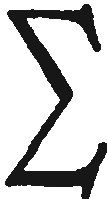
\includegraphics[scale=0.09]{FOTOS/Sigma.png}}}
% \setlength{\parindent}{0mm}
% )))

% === ITALICA EN ENTORNO MATEMÁTICO === (((
% \DeclareSymbolFont{italics}{\encodingdefault}{\rmdefault}{m}{it}
% \DeclareSymbolFontAlphabet{\mathit}{italics}
% \ExplSyntaxOn
% \int_step_inline:nnnn { `A } { 1 } { `Z }
 % {  \exp_args:Nf \DeclareMathSymbol{\char_generate:nn{#1}{11}}{\mathalpha}{italics}{#1} }
% \int_step_inline:nnnn { `a } { 1 } { `z } {  \exp_args:Nf \DeclareMathSymbol{\char_generate:nn{#1}{11}}{\mathalpha}{italics}{#1}}
% \ExplSyntaxOff
% )))

\begin{document}

\frame{\titlepage}

\begin{frame}[t]
	\begin{block}{}
		El concepto de un movimiento armónico simple no es realista, a menos que la masa esté colgada en un vacío perfecto, ya que al menos bará una fuerza de resistencia debida al medio que lo rodea.
		En mecánica, se considera que las fuerzas de amortiguamiento que actúan sobre un cuerpo son proporcionales a alguna potencia de la velocidad instantánea.
		En particular, supondremos que ésta fuerza es proporcional a la derivada de \(x\) con respecto al tiempo.
		\begin{minipage}{0.4\linewidth}
			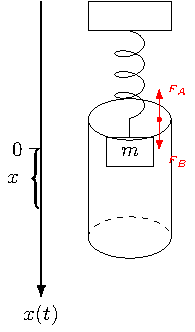
\includegraphics[width= 0.6 \linewidth]{IMAGENES/1/tikz.pdf}
		\end{minipage}\hspace{5mm}
		\begin{minipage}{0.5\linewidth}
			La fuerza total que se ejerce sobre la masa es:
			\[
				F_T = -kx- \beta x'.
			\]
			Por la \(2^{da}\) Ley de Newton \(F_T=ma=mx'\). \\[2mm]
			Por lo cual, se tiene
			\[
				mx'' = -kx - \beta x'.
			\]
		\end{minipage}
	\end{block}
\end{frame}

\begin{frame}[t]
	\begin{block}{}
		\[
			\begin{array}{rrcl}
				\iff & mx'' + \beta x' + kx & = & 0 \\[2mm]
				\iff & x'' + 2 \lambda x' + \omega ^2x & = & 0.\\
			\end{array}
		\]
		\[
			\underbrace{\hphantom{x'' + 2 \lambda x' + \omega ^2x = 0}}_\text{\color{red} E.D.O. de \(2^{do}\) Orden lineal homogénea coef. const.} 
		\]
		donde \(2 \lambda = \beta /m\), \(\omega ^2 = k/m\). \\[2mm]
		Esta E.D. está sujeta a la C.I. \(x(0) = x_0\), \(x' (0) = x_1\).
		Resolvemos este P.V.I., usando la ecuación característica:
		\[
			m^2+2 \lambda m + \omega ^2 =0.
		\]
		\[
			\begin{array}{rcl}
				m_{1,2} & = & \dfrac{-2 \lambda \pm \sqrt{(2 \lambda) ^2 - 4(\omega ^2)}}{2}\\[2mm]
				& = & - \lambda \pm \sqrt{\lambda ^2- \omega ^2} .
			\end{array}
		\]
		Se tienen \(3\) casos.
	\end{block}
\end{frame}

\begin{frame}[t]
	\begin{block}{}
		\begin{enumerate}
			\item \fbox{\(\lambda ^2- \omega ^2 >0\)} raíces reales y distintas negativas \(m_1,m_2\) 
				\[
					\begin{array}{c}
						x(t) = c_1e^{m_1t} + c_2e^{m_2t}. \\[2mm]
						\dis\lim_{t\rightarrow \infty} x(t) =0. \mbox{la masa tiende al equilibrio resorte.}
					\end{array}
				\]
				\begin{minipage}{0.4\linewidth}
					chales
				\end{minipage}\hspace{5mm}
				\begin{minipage}{0.5\linewidth}
					chales 2
				\end{minipage}
		\end{enumerate}
	\end{block}
\end{frame}

\end{document}
